\documentclass[10pt,a4paper]{article}
\usepackage{amsmath,graphicx,subfigure, hyperref, url}

\title{{Master Thesis\\[0.5em]}
       {\bf \huge Development of a game for hand- and eye coordination in children rehabilitation.\\[0.5em]}
       {\bf Weekly Report 10}}
\author{Anna Maria Walach, S121540}
\setlength{\parindent}{0mm}
\setlength{\parskip}{\medskipamount}

\begin{document}

\maketitle

\section*{What has been done this week}
During last week, I tried to discover if Myo is appropriate device for kids and come up with the test scenario and game description. 
\subsection*{Test scenario}
Each test should have three phases:
\begin{enumerate}
\item \emph{Calibration} - adjusting the device to the user.
\item \emph{Warm-up} - 5-15 minutes of casual movement and playing around with the device to get used to it, finalized with resynchronization. 
\item \emph{Playing the game} - 20-40 minutes session of playing the game.
\end{enumerate}

Following topics should be evaluated during the test session:
\begin{itemize}
\item how much user enjoyed the game?
\item how many progress was he able to accomplish per time unit?
\item what is the ratio of recognized gestures to all gestures?
\item what is the average "travelling" distance?
\end{itemize}

Following conditions should be possible to be fulfilled during training session:
\begin{itemize}
\item user should do at least 10 gestures per minute
\item user should actively use his arm
\item game should provide cognitive aspect
\end{itemize}

Based on prepared test scenario, following game description was created:

\begin{figure}[ht]
\centering
\includegraphics[width=\textwidth]{drawing.png} 
\caption{Concept art from the game "Battle of the Rainbow Bridge (2015).}
\label{fig:screen}

\end{figure}

\subsection*{Game description}
The game is called "Battle of the Rainbow Bridge". In the game player is a wizard, defending the bridge from the monsters.
Picture \ref{fig:screen} shows the game view. We can see three different type of items:
\begin{itemize}
\item \emph{wand} (red-brown shape) - the wand may be waved around, but it acts like extension of its bottom end was attached to the edge of the screen, so the movement is similar to movement of an arm if elbow is on the table.
\item \emph{cubes} - cubes represents monster and are coming to the player along different axis of cone with 120 degrees inner angle, where the top of the cone is a little bit higher then the middle of bottom edge of screen. 
\item \emph{laser} (three purple ribbons) - laser is shot from the wand, may have different colors depending on shooting command (gesture - fist, finger spread, wave in, wave out, pitch).
\end{itemize}

The player is not changing his position, only waves the wand. In order to shot a monster, player needs to hit it with a spell of the same colour as a monster.

The game allows gradual progress - on first level, monsters are slow and player knows only one spell. When player advances, next levels have faster monsters. After defeating them, player learns new spell (gesture) and the monsters are slow again. This process repeats, until player masters all five spells and defeats extremely fast monsters.

If player lose the level, game will try to lower the difficulty, with some kind of encouraging message "I see it's not your day, let's try with different monsters?" 

I am also considering an option with two hands involved in the game - one controlling position of the wand and one doing gestures - but it seem quite complicated (for a child).

\section*{Project status according to the study plan}
There is no delay in the plan (see updated plan, version 2). 

\section*{Plan for the next weeks}
Developing the game. 

\bibliographystyle{plainurl}
\bibliography{../thesis/bibliography/Bibliography}


\end{document}


% grammar check 
% make documentation!
% design the game
% make test requirements
% revise the study plan
% check for children usage on Google 
% write a mail to Rasmus
